%%%%%%%%%%%%%%%%%%%%%%%%%%%%%%%%%%%%%%%%%
% Beamer Presentation
% LaTeX Template
% Version 1.0 (10/11/12)
%
% This template has been downloaded from:
% http://www.LaTeXTemplates.com
%
% License:
% CC BY-NC-SA 3.0 (http://creativecommons.org/licenses/by-nc-sa/3.0/)
%
%%%%%%%%%%%%%%%%%%%%%%%%%%%%%%%%%%%%%%%%%

%----------------------------------------------------------------------------------------
%	PACKAGES AND THEMES
%----------------------------------------------------------------------------------------

\documentclass{beamer}

\mode<presentation> {

% The Beamer class comes with a number of default slide themes
% which change the colors and layouts of slides. Below this is a list
% of all the themes, uncomment each in turn to see what they look like.

%\usetheme{default}
%\usetheme{AnnArbor}
%\usetheme{Antibes}
%\usetheme{Bergen}
%\usetheme{Berkeley}
%\usetheme{Berlin}
%\usetheme{Boadilla}
%\usetheme{CambridgeUS}
%\usetheme{Copenhagen}
%\usetheme{Darmstadt}
%\usetheme{Dresden}
%\usetheme{Frankfurt}
%\usetheme{Goettingen}
%\usetheme{Hannover}
%\usetheme{Ilmenau}
%\usetheme{JuanLesPins}
%\usetheme{Luebeck}
\usetheme{Madrid}
%\usetheme{Malmoe}
%\usetheme{Marburg}
%\usetheme{Montpellier}
%\usetheme{PaloAlto}
%\usetheme{Pittsburgh}
%\usetheme{Rochester}
%\usetheme{Singapore}
%\usetheme{Szeged}
%\usetheme{Warsaw}

% As well as themes, the Beamer class has a number of color themes
% for any slide theme. Uncomment each of these in turn to see how it
% changes the colors of your current slide theme.

%\usecolortheme{albatross}
%\usecolortheme{beaver}
%\usecolortheme{beetle}
%\usecolortheme{crane}
%\usecolortheme{dolphin}
%\usecolortheme{dove}
%\usecolortheme{fly}
%\usecolortheme{lily}
%\usecolortheme{orchid}
%\usecolortheme{rose}
%\usecolortheme{seagull}
%\usecolortheme{seahorse}
%\usecolortheme{whale}
%\usecolortheme{wolverine}

%\setbeamertemplate{footline} % To remove the footer line in all slides uncomment this line
%\setbeamertemplate{footline}[page number] % To replace the footer line in all slides with a simple slide count uncomment this line

%\setbeamertemplate{navigation symbols}{} % To remove the navigation symbols from the bottom of all slides uncomment this line
}

\usepackage{graphicx} % Allows including images
\usepackage{booktabs} % Allows the use of \toprule, \midrule and \bottomrule in tables

%----------------------------------------------------------------------------------------
%	TITLE PAGE
%----------------------------------------------------------------------------------------

\title[]{Final Report} % The short title appears at the bottom of every slide, the full title is only on the title page

\author{Yan Song} % Your name
\institute[ISBD] % Your institution as it will appear on the bottom of every slide, may be shorthand to save space
{
ISBD \\ % Your institution for the title page
\medskip
 % Your email address
}
\date{\today} % Date, can be changed to a custom date

\begin{document}

\begin{frame}
\titlepage % Print the title page as the first slide
\end{frame}

\begin{frame}
\frametitle{Overview} % Table of contents slide, comment this block out to remove it
\tableofcontents % Throughout your presentation, if you choose to use \section{} and \subsection{} commands, these will automatically be printed on this slide as an overview of your presentation
\end{frame}

%----------------------------------------------------------------------------------------
%	PRESENTATION SLIDES
%----------------------------------------------------------------------------------------

%------------------------------------------------
 % Sections can be created in order to organize your presentation into discrete blocks, all sections and subsections are automatically printed in the table of contents as an overview of the talk
%------------------------------------------------
\section{Introduction}
\begin{frame}
\frametitle{Data Information}
\begin{itemize}
\item Sea surface temperature data collected by satellite.
\item Agulhas and surrounding areas off the coast of South Africa
\item January 1 to November 26, 2004, a period of 331 days.
\item A lot of missing values which were caused by land, satellite's orbital clipping and cloud cover.
\end{itemize}
\begin{figure}
\centering
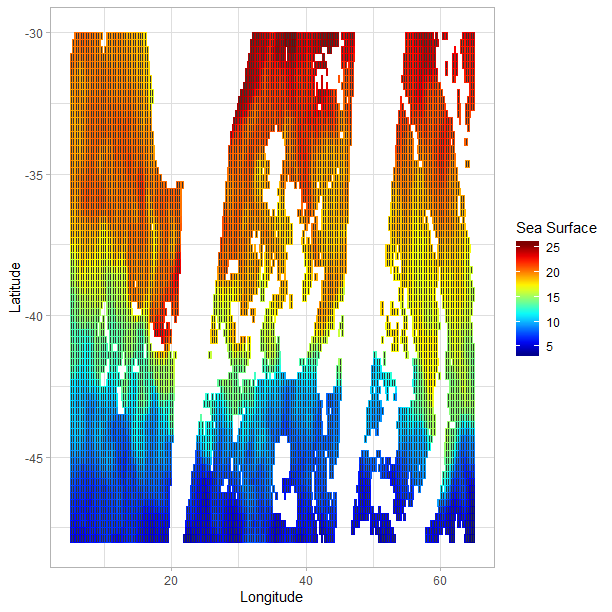
\includegraphics[scale=0.2]{Sea_surface_10.png}
\caption{Sea surface temperature on Day 10.}
\label{Figure 1}
\end{figure}
\end{frame}

\begin{frame}
\frametitle{Goal}
\begin{itemize}
\item \textbf{Goal}: Fill in the missing values of Day 10 data.
\item \textbf{Model}: Gaussian linear geostatistical model
\begin{equation*}
y(\mathbf{s}_i)=\mathbf{x}_i^T\beta+w(\mathbf{s}_i)+\epsilon_i,\quad\epsilon_i\stackrel{\text{i.i.d}}{\sim}\mathrm{N}(0,\tau^2)
\end{equation*}
\begin{equation*}
\mathbf{y}\sim\mathrm{N}(X\beta,\Sigma(\theta)),
\end{equation*}
where the $(i,j)$th element of $\Sigma(\theta)$ is $\sigma^2\exp{\{-\frac{\|\mathbf{s}_i-\mathbf{s}_j\|}{\phi}\}}+\tau^2\mathbf{1}(\mathbf{s}_i=\mathbf{s}_j)$
\item \textbf{Limitation}: Gaussian geostatistical model need $O(n^3)$ numerical operations to estimate parameters and make prediction. It is time consuming.
\end{itemize}
\end{frame}

\begin{frame}
\frametitle{Solution}
\begin{itemize}
\item \textbf{Solution}: Consider a data reduction.
\item \textbf{Following section}:
\begin{itemize}
\item Introduce three subsampling methods: Random, Deep and Wide, and MaxProLHD.
\item Compare the performance of various methods in parameter estimation and prediction.
\item Choose a subsampling method and use it to fill in the missing value.
\end{itemize}
\end{itemize}
\end{frame}

\section{Subsampling Methods}
\begin{frame}
\frametitle{Random}
Choose $m$ subsamples randomly from full data.
\begin{figure}
\centering
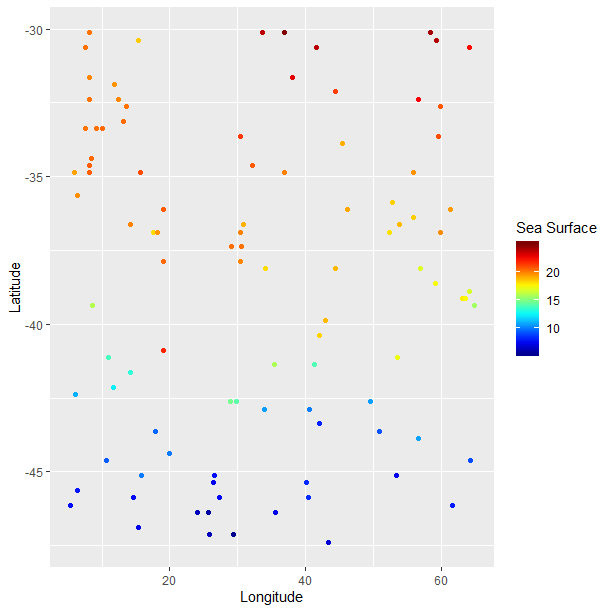
\includegraphics[scale=0.25]{Rsubsamples_darktheme.png}\\
\caption{100 Random subsamples}
\label{Figure 2}
\end{figure}
\end{frame}

\begin{frame}
\frametitle{Deep and Wide (DaW)}
\begin{itemize}
\item Step 1: Choose five subsamples randomly, called center points (Wide).
\item Step 2: For each center point, choose its $\frac{m}{5}-1$ nearest subsamples (Deep).
\end{itemize}
\begin{figure}
\begin{center}
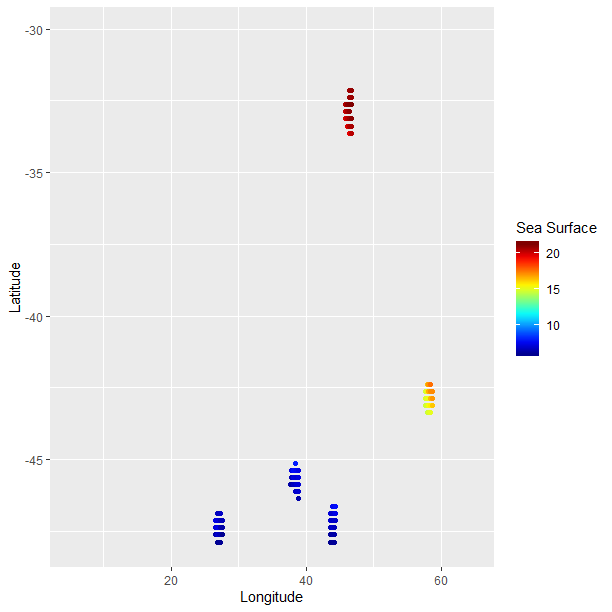
\includegraphics[scale=0.25]{DAWsubsamples_darktheme.png}\\
\caption{100 DaW subsamples}
\label{Figure 3}
\end{center}
\end{figure}
\end{frame}

\begin{frame}
\frametitle{Maximum Projection Design (MaxPro)}
\begin{itemize}
\item Step 1: Generete $m$ MaxPro design points by R package \emph{MaxPro}.
\item Step 2: Select the nearest neighbor for each design point from full data.
\end{itemize}
\begin{figure}
\begin{center}
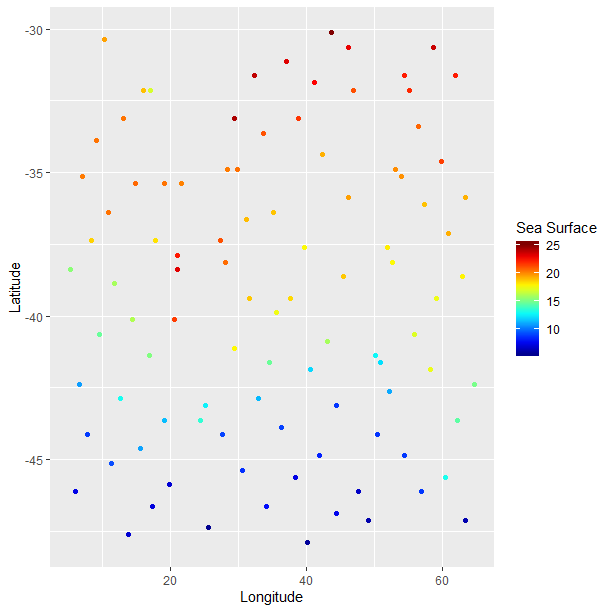
\includegraphics[scale=0.25]{MAPsubsamples_darktheme.png}\\
\caption{100 MaxPro subsamples}
\label{Figure 4}
\end{center}
\end{figure}
\end{frame}

\section{Subsampling Methods Comparison}
\begin{frame}
\frametitle{Agorithm}
The algorithm is summarized as follows.
\begin{itemize}
\item Step 1: Divide the full data into two parts, a random subset of 4000 observations as the training set and the remaining 6945 observations as the test data.
\item Step 2: Estimate the parameters and predict the test data with training set, or "full data". Treat the results as standards.
\item Step 3: Choose $m$ subsamples from "full data" by various subsampling methods, where $m$=100, 200 and 300. Utilize subsamples to estimate the parameters and predict the test data.
\item Step 4: Repeat step 3 100 times.
\end{itemize}
\end{frame}

\begin{frame}
\frametitle{Parameter Estimation: Trend Parameters}
\begin{figure}
  \centering
  % Requires \usepackage{graphicx}
  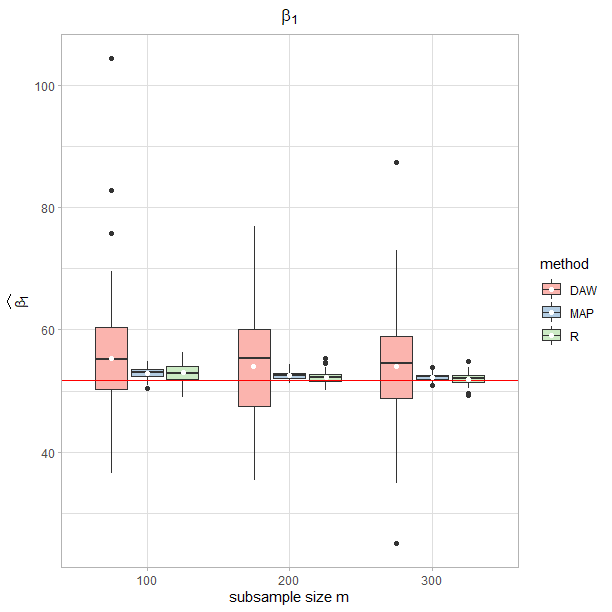
\includegraphics[scale=0.3]{beta1_boxplot.png}\\
  \caption{Boxplot of $\hat{\beta}_1$ estimated by various subsampling methods under m=100,200 and 300.}\label{Figure 5.1}
\end{figure}
\end{frame}

\begin{frame}
\frametitle{Parameter Estimation: Covariance Parameters}
\begin{figure}
  \centering
  % Requires \usepackage{graphicx}
  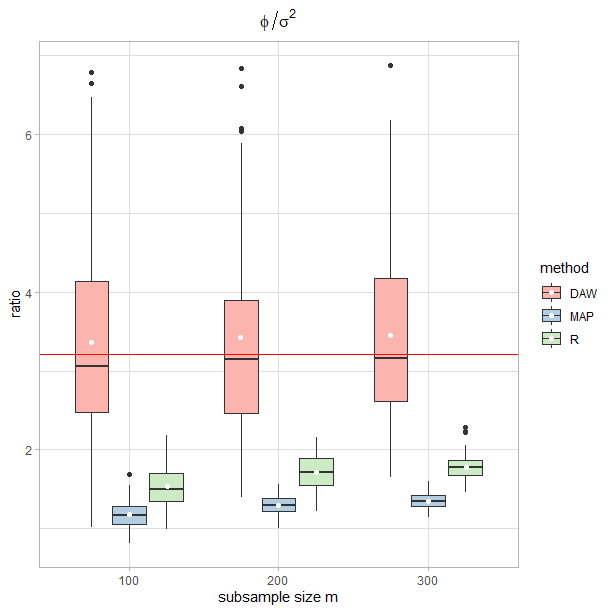
\includegraphics[scale=0.3]{ratio_boxplot.png}\\
  \caption{Boxplot of $\phi/\sigma^2$ estimated by various subsampling methods under m=100,200 and 300.}\label{Figure 5.2}
\end{figure}
\end{frame}

\begin{frame}
\frametitle{Parameter Estimation: Nugget Effect}
\begin{figure}
  \centering
  % Requires \usepackage{graphicx}
  \includegraphics[scale=0.3]{tausq_boxplot.png}\\
  \caption{Boxplot of $\tau^2$ estimated by various subsampling methods under m=100,200 and 300.}\label{Figure 5.3}
\end{figure}
\end{frame}

\begin{frame}
\frametitle{Parameter Estimation: Total MSEs}
\begin{figure}
  \centering
  % Requires \usepackage{graphicx}
  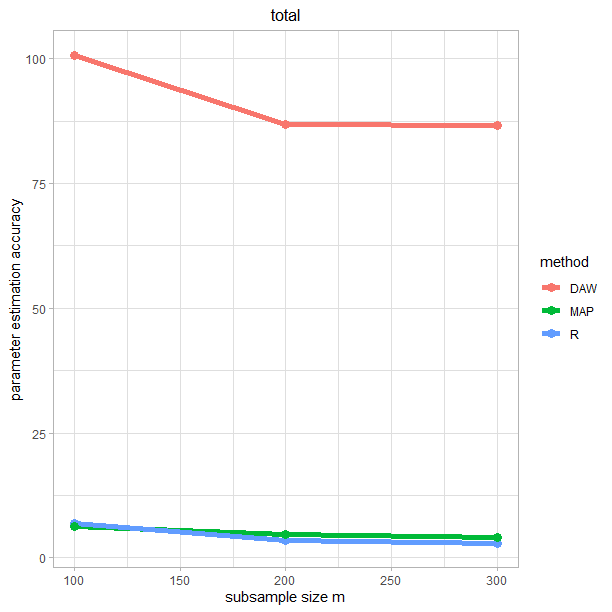
\includegraphics[scale=0.3]{total_mse.png}\\
  \caption{The sum of all parameters' MSEs}\label{Figure 5.1}
\end{figure}
\end{frame}

\begin{frame}
\frametitle{Prediction}
\begin{figure}
  \centering
  % Requires \usepackage{graphicx}
  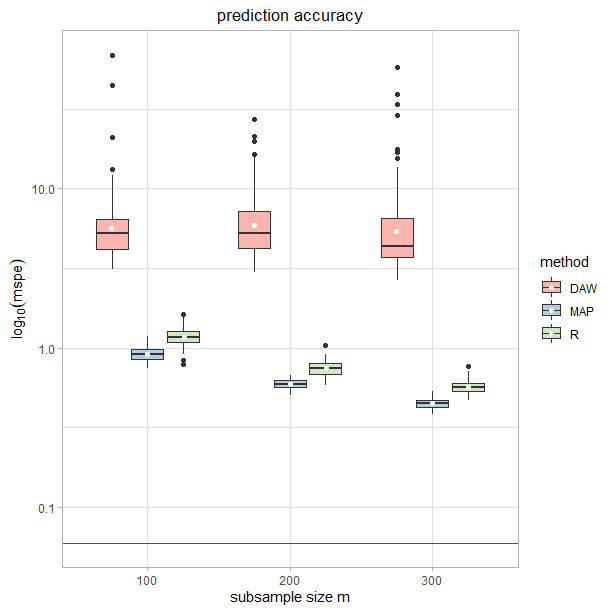
\includegraphics[scale=0.3]{pa_boxplot.png}\\
  \caption{Boxplot of prediction accuracy of various subsamples.}\label{Figure 6}
\end{figure}
\end{frame}

\section{Fill in Missing Values}
\begin{frame}
\frametitle{Fill in Missing Values}
\begin{figure}
  \centering
  % Requires \usepackage{graphicx}
  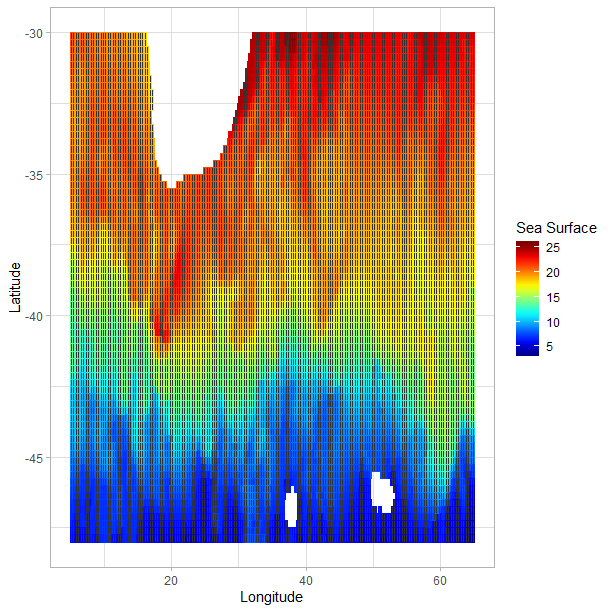
\includegraphics[scale=0.25]{Sea_fill_300.png}
  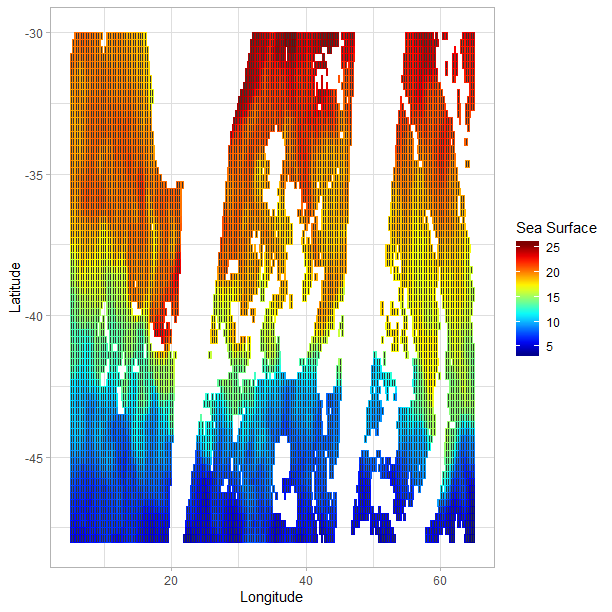
\includegraphics[scale=0.25]{Sea_surface_10.png}\\
  \caption{Sea surface temperatures on Day 10.}\label{Figure 7}
\end{figure}
\end{frame}

\section{Discussion}
\begin{frame}
\frametitle{Subsampling Method}
\begin{itemize}
\item MaxPro: 
\begin{itemize}
\item trend parameters, prediction.
\item computational limitation.
\end{itemize}
\item Deep and Wide:
\begin{itemize}
\item covariance parameters 
\item large variance $\to$ ensemble
\end{itemize}
\item Random:
\begin{itemize}
\item is close to MaxPro.
\item can be used when we want to fill in missing values quickly and easily.
\end{itemize}
\item Missing values in data of other days can be filled in by MaxPro.
\item The selection of subsampling method based on data and our target.
\end{itemize}
\end{frame}


%----------------------------------------------------------------------------------------

\end{document}

